\section{磁感应强度与磁场的空间描述}
静磁场由稳恒电流产生。这里的“稳恒”要求空间各处的电流密度不随时间改变，导体表面的电荷分布也已经建立；它并不要求单个载流子静止。研究磁场时应分清电流元所在的位置与场点所在的位置：前者决定积分变量，后者在一次积分中保持不动。


磁感应强度 $\bm B$ 是矢量。试探电荷以不同方向运动时受到的磁力不同，因此不能只用一个力除以一个电荷就定义磁场的全部性质。对于速度垂直于场的正电荷，磁力大小满足 $F=qvB$，方向再由叉乘确定。单位特斯拉满足 $\mathrm T=\mathrm{N/(A\,m)}$。后面的力学问题以给定磁场为条件，本讲先研究电流怎样决定这个场。


磁场叠加发生在同一个场点。两条导线产生的场即使大小相等，也只有方向相反才能抵消；不能把两个大小相减后得到零，就认定该处没有磁场。作图时先画从电流到场点的位置矢量，再画与它垂直的磁场方向，往往比直接套“顺时针”更可靠。

\fig{fig:mg1:k:vector}{电流元、场点与磁场的方向}{\begin{tikzpicture}[scale=.88]
\draw[world](-1,0)--(1,0);\draw[flow](-.8,0)--(.5,0)node[midway,below]{$I\dd\bm l$};\fill(0,0)circle(2pt)node[above left]{$A$};\fill(2.8,1.8)circle(2pt)node[right]{$P$};\draw[flow](0,0)--(2.8,1.8)node[midway,above]{$\bm r$};\node at(2.8,2.5){$\odot\,\dd\bm B$};
\end{tikzpicture}}
\section{毕奥—萨伐尔定律与积分变量}
图\ref{fig:mg1:k:vector}中 $\bm r$ 从电流元指向场点，真空中有
\begin{equation}\dd\bm B=\frac{\mu_0 I}{4\pi}\frac{\dd\bm l\times\bm r}{r^3},
\qquad \bm B(P)=\frac{\mu_0}{4\pi}\int\frac{\bm J(\bm r')\times(\bm r-\bm r')}{|\bm r-\bm r'|^3}\dd V'.\end{equation}
第一式适合细导线，第二式把电流密度分布纳入同一框架。这里 $\mu_0$ 为真空磁导率。电流元不是可以独立存在的稳恒电流，实际回路还应满足电流连续；把某一段导线单独积分，是计算完整回路的一部分贡献。


先看沿 $z$ 轴的直线段，场点到轴的垂距为 $a$，垂足取 $z=0$。每一电流元的场都沿同一环向，因此可先确定方向，再积大小。由 $r^2=a^2+z^2$、$\sin\theta=a/r$，得到

\[
B=\frac{\mu_0 I}{4\pi}\int_{z_1}^{z_2}\frac{a\,\dd z}{(a^2+z^2)^{3/2}}
=\frac{\mu_0I}{4\pi a}\left[\frac{z}{\sqrt{a^2+z^2}}\right]_{z_1}^{z_2}.
\]
原函数可由三角换元得到：令 $z=a\tan\alpha$，
$\dd z=a\sec^2\alpha\dd\alpha$，其中 $-\pi/2<\alpha<\pi/2$，故
\[
 \frac{a\dd z}{(a^2+z^2)^{3/2}}=\frac{\cos\alpha}{a}\dd\alpha,
 \qquad
 \int\frac{\cos\alpha}{a}\dd\alpha
 =\frac{\sin\alpha}{a}
 =\frac{z}{a\sqrt{a^2+z^2}}.
\]
上下限分别变为 $\alpha_j=\arctan(z_j/a)$，便有 $B=\mu_0I(\sin\alpha_2-\sin\alpha_1)/(4\pi a)$。端点分居垂足两侧时两个角一正一负，结果表现为两个正弦的和；垂足在延长线上时应保留有向角，不能仍照抄“相加”。


取两端分别趋于负无穷与正无穷，得到长直导线 $B=\mu_0I/(2\pi a)$。只留一侧半无限导线时，结果减半。这些系数来自积分边界，而不是由图形看起来“很长”决定。实际长度是否足够大，可以用有限长度结果估计误差。

\fig{fig:mg1:k:wire}{有限直导线的有向端点角}{\begin{tikzpicture}[scale=.88]
\draw[world](0,-1.7)node[left]{$z_1$}--(0,2.4)node[left]{$z_2$};\draw[flow](0,1)--(0,1.8)node[left]{$I$};\fill(3,0)circle(2pt)node[right]{$P$};\draw[guide](0,0)--(3,0);\draw[guide](0,-1.7)--(3,0)--(0,2.4);\node at(1.3,-.3){$a$};\node at(2.15,.3){$\alpha_2$};\node at(2,-.6){$\alpha_1$};
\end{tikzpicture}}

图\ref{fig:mg1:k:wire}的两个端点角都从垂足方向量起，分别保留正负。积分原函数的上端减下端因此统一适用于垂足在线段内外两类情形；端点移到同一侧时，不可继续把两正弦无条件相加。


\subsection{圆弧、圆环与轴线上的场}
圆弧中心到每个电流元的距离都为 $R$，且 $\dd\bm l\perp\bm r$。圆心场的方向处处一致，弧长元为 $R\dd\varphi$，所以
\[
 B=\frac{\mu_0I}{4\pi R}\int_0^\varphi\dd\theta
 =\frac{\mu_0I}{4\pi R}[\theta]_0^\varphi
 =\frac{\mu_0I\varphi}{4\pi R},
\]这里的角度必须以弧度代入。径向导线对圆心的贡献为零，因为其电流元与位置矢量共线；这并不意味着任意引线都可以忽略。


计算完整圆环轴线上的场时，各电流元的场大小相等，但方向并不相同。横向分量由对称电流元两两抵消，只有轴向分量叠加。若轴向坐标为 $x$，距离 $s=\sqrt{R^2+x^2}$，则 $\dd B_x=\mu_0I R\,\dd l/(4\pi s^3)$，积分得

\[
B_x=\frac{\mu_0IR^2}{4\pi(R^2+x^2)^{3/2}}\int_0^{2\pi}\dd\varphi
=\frac{\mu_0IR^2}{4\pi(R^2+x^2)^{3/2}}[\varphi]_0^{2\pi}
=\frac{\mu_0IR^2}{2(R^2+x^2)^{3/2}}.
\]
在圆心它回到 $\mu_0I/(2R)$；在 $|x|\gg R$ 处它按 $|x|^{-3}$ 衰减。把磁矩 $m=I\pi R^2$ 代入，远轴场写成 $\mu_0m/(2\pi|x|^3)$。相同的远场尺度解释了小线圈的磁偶极近似，但近场仍应按实际导线积分。

\fig{fig:mg1:k:ring}{圆环轴线上，对称电流元的横向场抵消，轴向场同向叠加}{\begin{tikzpicture}

\draw[axis](-1,0)--(6.2,0)node[right]{$x$};\draw[world](0,0)ellipse(.65 and 1.8);
\fill(0,1.8)circle(1.7pt)node[above]{$A$};\fill(0,-1.8)circle(1.7pt)node[below]{$A'$};\fill(3,0)circle(1.7pt)node[below]{$P$};
\draw[guide](0,1.8)--(3,0)--(0,-1.8);\draw[dim](-.9,0)--(-.9,1.8)node[midway,left]{$R$};
\draw[dim](0,-2.3)--(3,-2.3)node[midway,below]{$x$};\node at(1.2,1.35){$s$};
\draw[->,blue,thick](3,0)--(4.8,3)node[above]{$\dd\bm B_A$};\draw[->,blue,thick](3,0)--(4.8,-3)node[below]{$\dd\bm B_{A'}$};
\draw[guide](4.8,3)--(4.8,-3);\draw[->,red,very thick](3,0)--(4.8,0)node[midway,above]{$\dd B_x$};
\node[above,align=center]at(0,2.7){$A:\odot I\dd l$};\node[below,align=center]at(0,-3.1){$A':\otimes I\dd l$};
\node[align=center]at(3.4,4){$\dd B_x=\dd B\,R/s$\\$\dd B=\mu_0I\dd l/(4\pi s^2)$};

\end{tikzpicture}}
图\ref{fig:mg1:k:ring}采用经过轴线的截面，圆环用透视椭圆表示。上、下电流元的方向分别向纸外、纸内；两条蓝箭头都垂直于各自指向 $P$ 的位置矢量。由直角三角形，磁场与轴向夹角的余弦是 $R/s$，不是 $x/s$，因此保留下来的轴向微元为 $\dd B_x=\mu_0IR\dd l/(4\pi s^3)$。先消去横向分量，再沿圆周积分，才得到上式中的 $R^2$ 因子。



\section{运动电荷、面电流与分布电流}
在低速、准静态近似下，运动点电荷的磁场为 $\bm B=\mu_0q\,\bm v\times\bm r/(4\pi r^3)$。这个表达式强调电流与电荷运动之间的联系；对于快速变化的运动，场还涉及传播延迟，不能把此式当作任意时刻的精确规律。


旋转带电体可按同心薄环分解。薄环上电量 $\dd q$ 每转一周通过一个固定截面一次，周期 $2\pi/\omega$，故 $\dd I=\omega\dd q/(2\pi)$。先求这一电流，再用圆环场积分，避免把整个圆盘都按外缘速度处理。若体电流密度为 $\bm J$，则穿过微小截面的电流为 $\bm J\cdot\dd\bm S$；若电流集中在薄面内，面电流密度 $\bm K$ 的单位为 $\mathrm{A/m}$。


把许多细导线排列成面电流时，还需交代观察尺度。导线间距为 $d$，只有在距线排的高度远大于 $d$，或题目已明确作连续面模型时，才可把离散电流平滑为 $K=I/d$。紧贴某根细线时仍出现局部的 $1/r$ 场，连续模型无法描述这一细节。

\fig{fig:mg1:k:rotating}{旋转圆盘取窄环微元；连续面电流取垂直于电流方向的宽度}{\begin{tikzpicture}

\draw[world](0,0)circle(1.8);\fill[blue!15,even odd rule](0,0)circle(1.2)(0,0)circle(1.05);\draw(0,0)circle(1.2)(0,0)circle(1.05);
\draw[->](0,0)--(1.05,0)node[midway,below]{$r$};\draw[flow](1.5,.6)arc(22:100:1.62)node[above]{$\omega$};
\draw[flow](1.12,0)arc(0:90:1.12);\node at(0,-2.3){$\dd q=\sigma\,2\pi r\dd r$};\node at(0,-2.9){$\dd I=\omega\sigma r\dd r$};
\draw[flow](1.7,1.7)--(.84,.84)node[pos=0,above right]{$\dd r$};
\begin{scope}[xshift=5.8cm]
\fill[gray!10](-1.6,-1.6)rectangle(1.6,1.6);\foreach \y in {-1.2,-.6,0,.6,1.2}{\draw[flow](-1.4,\y)--(1.4,\y);}
\draw[dim](2,-.6)--(2,.6)node[midway,right]{$\dd w$};\node at(0,2.15){面电流 $\bm K$};\node at(0,-2.3){$\dd I=K\dd w$};\node at(0,-2.9){$[K]=\mathrm{A/m}$};
\end{scope}

\end{tikzpicture}}
图\ref{fig:mg1:k:rotating}左侧窄环的半径 $r$ 是积分变量，环宽为 $\dd r$；每一圈包含的电量乘旋转频率才给出该窄环的等效电流。求圆心场时，再将 $\dd I$ 代入 $\dd B=\mu_0\dd I/(2r)$，这里一个 $r$ 会约去。右侧的 $\dd w$ 沿面内、垂直于电流方向量取，故面电流的电流元是 $K\dd w$，不能误乘沿电流的路径长度。



\section{磁通量与磁场的无源性质}
磁感线是在每一点与 $\bm B$ 相切的几何曲线，疏密只是辅助表示大小。没有磁单极源意味着任意闭合曲面穿出的有向磁通为零，
\[
\oint_S\bm B\cdot\dd\bm S=0.
\]
闭合曲面的法线统一向外；一个面上的正通量可由其他面上的负通量抵消。磁感线可以形成闭环，也可以延伸到无穷远，不能据此把均匀场中的每一条直线都画成有限闭环。


开曲面须先选正法线，磁通为 $\Phi=\int_S\bm B\cdot\dd\bm S$。只有平面内磁场均匀时，才能写成 $BS\cos\theta$。若场随位置变化，应同时保留场的空间函数和面积元；长直导线穿过邻近矩形面的磁通便会含有对数。两个以同一闭合边界为边缘、方向约定相容的曲面，磁通相同，因为它们合成的闭合曲面总通量为零。这个结论将为电磁感应中的选面提供依据。

\fig{fig:mg1:k:flux}{长直导线邻近矩形面的磁通必须保留随距离变化的磁场}{\begin{tikzpicture}

\draw[world](0,-.6)--(0,3.8);\draw[flow](0,2.2)--(0,3.2)node[left]{$I$};
\fill[blue!8](1,0)rectangle(4.2,3);\draw[world](1,0)rectangle(4.2,3);\fill[orange!25](2.4,0)rectangle(2.7,3);\draw(2.4,0)--(2.4,3)(2.7,0)--(2.7,3);
\foreach \x in {1.4,2,3.1,3.8}\foreach \y in {.5,1.5,2.5}{\node at(\x,\y){$\otimes$};}
\draw[axis](0,-1)--(5,-1)node[right]{$r$};\node[below]at(1,-1){$a$};\node[below]at(4.2,-1){$b$};
\draw[dim](4.7,0)--(4.7,3)node[midway,right]{$L$};\node[above]at(2.55,3.25){$\dd r$};
\node at(2.5,4){正法线取向纸内：$\bm n=\otimes$};\node at(2.5,-1.8){$\dd S=L\dd r,\quad B(r)=\mu_0I/(2\pi r)$};

\end{tikzpicture}}
图\ref{fig:mg1:k:flux}中，导线右侧的磁场向纸内，与所选正法线同向。取窄条而非整块矩形作面积元，是因为同一条内磁场不随纵向位置改变，而不同条的 $r$ 不同。因此

\[
 \Phi=\int_a^b\frac{\mu_0I}{2\pi r}L\dd r
 =\frac{\mu_0IL}{2\pi}[\ln r]_a^b
=\frac{\mu_0IL}{2\pi}(\ln b-\ln a)
=\frac{\mu_0IL}{2\pi}\ln\frac ba.
\]
若把法线反向，整个结果变号；若矩形宽度 $b-a\ll a$，才可用近似均匀场 $B(a)$ 得到 $\Phi\simeq B(a)L(b-a)$。对数式与这一窄面极限相容。



\section{安培环路定理及其使用条件}
在真空稳恒电流条件下，沿闭合路径 $C$ 有
\begin{equation}\oint_C\bm B\cdot\dd\bm l=\mu_0I_{\text{穿过}}.\end{equation}
路径的绕行方向决定右手正法线，穿过面的电流按正负相加。右端只计穿过面内的电流，左端的 $\bm B$ 却由空间全部电流共同决定。因此，回路中没有净电流，只能推出环量为零，不能推出沿路每一点的场为零。


长直电流的圆形环路给出 $B\,2\pi r=\mu_0I$，这里能够把 $B$ 提到积分号外，依靠绕轴旋转对称；场沿圆周切向则来自右手方向及轴向平移对称。若电流分布没有足够对称性，环路定理仍然成立，却可能不能独立解出各处的场。


还可从毕奥—萨伐尔积分理解一般结论。对闭合载流导线与观察回路作双重积分，交换积分次序后，几何因子可解释为载流回路相对观察点扫过面的有向立体角变化。一次正向穿过使变化量为 $4\pi$，反向穿过使其为 $-4\pi$，未穿过的闭合电流贡献为零；再按电流叠加，得到右端的有向电流和。这样，圆形环路的计算揭示了系数，一般闭合回路的穿绕关系则解释了为何结果不依赖所选曲面的形状。


对随时间变化且存在位移电流的情形，单独使用上述稳恒形式会遇到选面矛盾。本专题的环路计算均在稳恒条件下进行；电磁感应与交流电中涉及电容极板间的场时，需要加入相应的位移电流项。

\fig{fig:mg1:k:ampere}{从正法线一侧观察，环路逆时针时，向纸外电流计正}{\begin{tikzpicture}

\draw[world](0,0)ellipse(2.2 and 1.5);\draw[flow](1.555,1.061)arc(45:130:2.2 and 1.5);
\node[above]at(0,2.1){$\bm n=\odot$，$C$ 逆时针};
\node at(-.85,0){$\odot$};\node[below]at(-.85,-.3){$I_1$};\node at(.85,0){$\otimes$};\node[below]at(.85,-.3){$I_2$};
\node at(0,-2.25){$I_{\text{穿过}}=I_1-I_2$};\node at(3.3,.5){$\odot I_3$};\node[align=center]at(3.3,-.6){回路外电流\\不计入右端};

\end{tikzpicture}}

图\ref{fig:mg1:k:ampere}先规定环路正向及右手法线，再按穿面电流方向得到 $I_1-I_2$。即使两项相等、净环量为零，回路上的局部场仍可能非零；必须有足够对称性才能把环量关系化成单个场值。


\section{平面、圆柱与螺线管的对称模型}
无穷面电流的场平行于面并垂直于 $\bm K$。镜面对称使两侧大小相同、方向相反。选跨过薄面的狭长矩形回路，两个长边各贡献 $BL$，得到 $B=\mu_0K/2$。方向可写为 $\bm B_+=\mu_0\bm K\times\bm n/2$，其中 $\bm n$ 指向“正侧”。两块面电流的场由矢量叠加决定；它们的电流相反时，夹层中的场增强，外侧抵消。


无限长圆柱电流具有绕轴对称，但内部环路只包围一部分电流。均匀电流密度 $J$ 时，$I_{\rm enc}=J\pi r^2$，因此内部 $B=\mu_0Jr/2$，外部按总电流写成 $\mu_0I/(2\pi r)$。在柱面处两式连续；若把内部也写成总电流除以 $2\pi r$，不仅中心发散，还违背电流包围关系。


理想无限长螺线管可看成绕圆柱面的连续环向面电流 $K=nI$。对称性使内部磁场沿轴，取同在管内、位于不同半径的两个轴向长边构成矩形，环路不穿过面电流，故两个长边的场相等。再取一个长边在外部的矩形，结合无穷远无外加场的边界条件，得到外部场为零、内部任意处 $B=\mu_0nI$。管内均匀并非仅由“轴线上知道一个数”推出，而是对称性、环路关系与边界条件共同给出的。有限长螺线管端部会出现边缘场，不能把无限长结论直接延伸到管口。


\fig{fig:mg1:k:symmetric}{环路中包围的电流随模型不同而改变，切向磁场由对称性确定}{\begin{tikzpicture}

\begin{scope}
\draw[world](0,0)circle(1.6);\fill[blue!10](0,0)circle(1.55);\draw[dashed](0,0)circle(.9);
\foreach \x/\y in {0/0,.6/.5,-.7/.5,.4/-1,-.7/-.8,1/.2}{\node at(\x,\y){$\odot$};}
\draw[flow](.9,0)arc(0:75:.9);\draw[dim](0,-.1)--(.9,-.1)node[midway,below]{$r$};\node at(0,2.2){均匀圆柱 $J$};\node at(0,-2.2){$I_{\rm enc}=J\pi r^2$};
\end{scope}
\begin{scope}[xshift=5.5cm]
\draw[very thick](-1.8,0)--(1.8,0);\foreach \x in {-1.5,-.75,0,.75,1.5}{\node at(\x,0){$\odot$};}
\draw[dashed](-1.6,-.8)rectangle(1.6,.8);\draw[flow](1,.8)--(-1,.8)node[midway,above]{$B$};\draw[flow](-1,-.8)--(1,-.8)node[midway,below]{$B$};
\node at(0,2.2){电流面 $K$ 向纸外};\node at(0,-2.2){$2BL=\mu_0KL$};\draw[dim](-1.6,-1.5)--(1.6,-1.5)node[midway,below]{$L$};
\end{scope}

\end{tikzpicture}}
图\ref{fig:mg1:k:symmetric}左侧圆环仅包围半径 $r$ 内的电流，故内部场随 $r$ 线性增加。右侧矩形的短边垂直于场，无环量贡献；上下长边沿环路正向都与各自的磁场同向，环量是 $2BL$。这两个模型能够直接求场，依赖的是已知的场方向与沿积分边的等模性质。




遇到偏心孔洞，可把实际电流分布看成完整圆柱的正电流密度，再在孔洞圆柱中叠加反向电流密度。对孔内点 $P$，位置矢量满足 $\bm r_1-\bm r_2=\bm a$，两项中的场点变量恰好消去，得到 $\bm B=\mu_0\bm J\times\bm a/2$。这是一种空间叠加产生的均匀场，不能把空洞中的电流为零误读为空洞中的磁场为零。

\fig{fig:mg1:k:cavity}{偏心孔洞中的正、负电流叠加}{\begin{tikzpicture}[scale=.88]
\draw[world](0,0)circle(2.2);\draw[world](.85,.3)circle(1.05);\fill(0,0)circle(1.5pt)node[below left]{$O_1$};\fill(.85,.3)circle(1.5pt)node[below right]{$O_2$};\fill(1.1,1)circle(2pt)node[right]{$P$};\draw[flow](0,0)--(.85,.3);\draw[guide](0,0)--(1.1,1)--(.85,.3);\node at(.1,.5){$\bm a$};\node at(-1.1,1.1){$\odot\bm J$};\node at(0,2.8){孔内叠加 $-\bm J$};
\end{tikzpicture}}

图\ref{fig:mg1:k:cavity}的两条辅助线都终止于同一场点 $P$。正、负圆柱电流的场分别依赖从 $O_1,O_2$指向 $P$的位矢；二者相减后只留下固定偏心矢量 $\bm a$，所以孔内场均匀，而非因孔内电流为零便没有场。



\section{有限螺线管与端部修正}
有限螺线管中的每一匝仍可按圆电流计算。设长度为 $l$，中点为轴向原点，半径 $R$，单位长度匝数 $n$。位于 $z'$ 到 $z'+\dd z'$ 的窄带包含 $n\dd z'$ 匝，轴上场点 $z$ 到该窄带的轴向距离为 $z-z'$，所以

\[
B_z(z)=\frac{\mu_0nIR^2}{2}\int_{-l/2}^{l/2}
\frac{\dd z'}{[R^2+(z-z')^2]^{3/2}}.
\]
把 $u=z-z'$ 作为新变量时，$\dd z'=-\dd u$，积分上下限也同时反向。原来的下限 $z'=-l/2$ 对应 $u=z+l/2$，上限 $z'=l/2$ 对应 $u=z-l/2$；负微分将次序交换。原函数来自
\[
 \frac{\dd}{\dd u}\left[u(R^2+u^2)^{-1/2}\right]
 =(R^2+u^2)^{-1/2}-u^2(R^2+u^2)^{-3/2}
 =\frac{R^2}{(R^2+u^2)^{3/2}}.
\]
于是 $B_z=(\mu_0nI/2)[u/\sqrt{R^2+u^2}]_{z-l/2}^{z+l/2}$，得到

\[
B_z(z)=\frac{\mu_0nI}{2}
\left[\frac{z+l/2}{\sqrt{R^2+(z+l/2)^2}}
-\frac{z-l/2}{\sqrt{R^2+(z-l/2)^2}}\right].
\]
这个表达式把长线圈的内部平台、管口过渡与外部衰减连在一起。对于远离两端且两端距离都远大于 $R$ 的内部点，两分式分别趋于1和 $-1$，场接近 $\mu_0nI$。在长线圈端口，只有一侧还近似延伸到无穷，场约为内部的一半。


因此“长度远大于半径”仍需与观察位置结合。即使线圈很长，管口附近也不满足无限长内部公式。作近似时可先把场点到近端的距离与 $R$ 比较，再决定是否保留端部修正。有限圆柱的外部场并非严格零；它与内部磁通相连，形成完整的无源场结构。

\fig{fig:mg1:k:finitecoil}{有限线圈由轴向窄带叠加}{\begin{tikzpicture}[scale=.88]
\draw[world](-2,-1)--(2,-1) (-2,1)--(2,1);\draw[world](-.2,-1)--(-.2,1) (.1,-1)--(.1,1);\draw[axis](-3,0)--(4,0)node[right]{$z$};\fill(3,0)circle(2pt)node[above]{$P$};\node[above]at(-.05,1.2){$n\,\dd z^{\prime}$ 匝};\node[below]at(-2,-1){$-l/2$};\node[below]at(2,-1){$l/2$};
\end{tikzpicture}}

图\ref{fig:mg1:k:finitecoil}中窄带含 $n\dd z'$匝，每匝到场点 $P$的轴向距离为 $z-z'$。求积分时改变的是窄带位置 $z'$，场点 $z$保持固定；端口处缺少另一侧的线圈贡献，正是长线圈端部场约减半的原因。


\section{近轴磁场的径向分量}
轴线上场随 $z$ 改变时，附近的场不能始终只有轴向分量。若只画一组疏密随高度改变却完全平行的磁感线，就会使上下横截面穿过的磁通不等，违背磁场无源性质。正确的近轴场还含小的径向分量，使磁感线向外展开或向内收拢。


在轴对称、轴附近无电流的区域，取半径 $r$、高 $\dd z$ 的小圆柱。上下两底的净通量约为 $\pi r^2B_0'(z)\dd z$，侧面通量约为 $2\pi r B_r\dd z$。闭合通量为零，给出

\[
B_r(r,z)=-\frac r2B_0'(z)+O(r^3).
\]
因此轴向场沿 $z$ 增强时，近轴径向场指向轴线；若轴向场减弱，则指向外侧。这个符号将直接用于磁镜的轴向平均力判断。

要进一步求轴向场的径向修正，在无电流区域使用小矩形环路的零环量，得到 $\partial B_r/\partial z=\partial B_z/\partial r$。将上一式对 $z$ 求导，得
$\partial_rB_z=-(r/2)B_0''(z)+O(r^3)$。以 $\rho$ 为径向积分变量，
\[
 B_z(r,z)-B_0(z)
 =-\frac{B_0''(z)}2\int_0^r\rho\dd\rho+O(r^4)
 =-\frac{B_0''(z)}2[\rho^2/2]_0^r+O(r^4).
\]
这里 $z$ 在径向积分中保持不变，得到

\[
B_z(r,z)=B_0(z)-\frac{r^2}{4}B_0''(z)+O(r^4).
\]
两个展开式说明，只要轴上函数足够光滑，就能求出邻近空间的最低阶结构。展开要求 $r$ 远小于轴向变化尺度，而且整个小区域内不能穿过电流面；不能把这个无电流关系跨过线圈绕组直接延拓。对于双线圈中心，若 $B_0'$ 与 $B_0''$ 同时为零，径向与轴向的低阶不均匀性会一起减弱，这解释了中心均匀场设计的三维意义。

\fig{fig:mg1:k:nearaxis}{小柱体的侧面磁通补偿两底磁通差，轴向增强的场必然向轴线收拢}{\begin{tikzpicture}

\draw[axis](0,-.9)--(0,3.5)node[above]{$z$};
\draw[->,blue,thick](-1.7,-.5)..controls(-1.4,1.6)and(-1.1,2.6)..(-.8,3.1);
\draw[->,blue,thick](1.7,-.5)..controls(1.4,1.6)and(1.1,2.6)..(.8,3.1);
\draw[world](0,.6)ellipse(1.15 and .25);\draw[world](-1.15,.6)--(-1.15,1.5)(1.15,.6)--(1.15,1.5);\draw[world](0,1.5)ellipse(1.15 and .25);
\draw[->,red,thick](1.15,1.05)--(.45,1.05);
\node[red,anchor=west]at(2.5,1.7){$B_r<0$};
\draw[dim](2,.6)--(2,1.5)node[midway,right]{$\dd z$};\draw[dim](0,.45)--(1.15,.45)node[midway,below]{$r$};
\node[right]at(2.5,2.6){$B_0(z+\dd z)$};\node[right]at(2.5,0){$B_0(z)$};
\node at(1,-1.5){$\pi r^2B_0'\dd z+2\pi rB_r\dd z=0$};

\end{tikzpicture}}

图\ref{fig:mg1:k:nearaxis}中上底穿出通量多于下底穿入通量，侧面就必须有净磁通穿入。正半径方向指向柱外，故其径向场为负，磁感线相应向轴线收拢。小柱体上下底的磁通差由侧面磁通抵消，这正给出 $B_r=-rB_0'/2$的符号与系数；只画逐渐变密的平行直线不能满足同一通量关系。


\section{电流面两侧的场与自身受力}
环路定理还能给出穿过理想薄电流面的边界关系。取法线 $\bm n$ 从负侧指向正侧，跨面矩形的高度趋零、长边仍有限，两个短边的环量趋零。由穿过矩形的面电流得到 $\bm n\times(\bm B_+-\bm B_-)=\mu_0\bm K$。另由极薄柱面的零总磁通，法向分量满足 $\bm n\cdot(\bm B_+-\bm B_-)=0$。


这两个条件分别限制切向场的跳变与法向场的连续。它们并不单独决定两侧各自的场，还需边界条件或对称性。例如叠加一个均匀外场后，跳变保持不变，两侧场却都改变。


计算薄电流面本身受到的力时，应使用其他电流产生的外场，不能直接使用包含自身贡献的某一侧总场。对对称薄层的极限，平均场 $(\bm B_++\bm B_-)/2$ 正好消去其反向自场，留下可用于 $\bm K\times\bm B_{\rm ext}$ 的场。这一规则解释了两层电流之间磁压力计算常见的因子二差异。


真实导体电流层具有有限厚度，场会在层内连续变化。薄层跳变、平均场受力都是对这一结构的极限描述。若给定的是体电流密度，就应先按厚度积分；若明确给定理想面电流，才直接使用跳变式。模型层次与单位的区别，需要在同一推导中始终保持。


\fig{fv:m1:sheet}{面电流的自场两侧反向，取平均才消去自场}{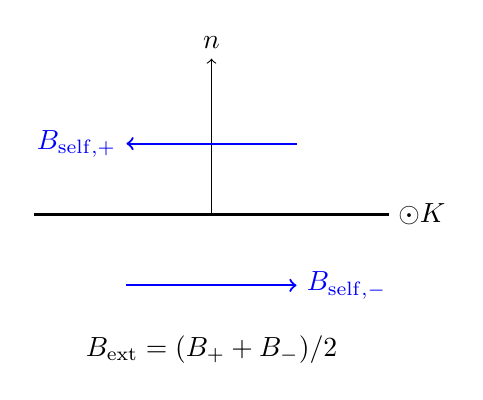
\begin{tikzpicture}[scale=.9]
\draw[very thick](-2.5,0)--(2.5,0);\node[right]at(2.5,0){$\odot K$};\draw[->](0,0)--(0,2.2)node[above]{$\bm n$};
\draw[->,blue,thick](1.2,1)--(-1.2,1)node[left]{$\bm B_{\rm self,+}$};
\draw[->,blue,thick](-1.2,-1)--(1.2,-1)node[right]{$\bm B_{\rm self,-}$};
\node at(0,-1.9){$\bm B_{\rm ext}=(\bm B_++\bm B_-)/2$};\end{tikzpicture}}
图\ref{fv:m1:sheet}取面电流向纸外、正法线向上，右手关系给上方自场向左、下方向右。叠加同一个平滑外场后，两侧总场之差保留自场的跳变，平均值则消去这对反向贡献。计算面本身受力所需的正是剩下的外场，而非任意一侧总场。这把环路的边界关系与薄层机械受力联系起来，也说明用层间总场求单层力为何容易多算一倍。


\section{零场点邻域的几何结构}
零场点不是场方向任意的一小片均匀区域。以两条位于 $(\pm a,0)$ 的同向相等电流为例，在两线中点附近，令 $c=\mu_0I/(2\pi)$，两线精确场为
\[
 \bm B=c\left[
 \frac{-y\bm e_x+(x-a)\bm e_y}{(x-a)^2+y^2}
 +\frac{-y\bm e_x+(x+a)\bm e_y}{(x+a)^2+y^2}\right].
\]
当 $|x|,|y|\ll a$，利用 $(1+\epsilon)^{-1}=1-\epsilon+O(\epsilon^2)$，
两分母的倒数分别为 $a^{-2}(1+2x/a)+O((x^2+y^2)/a^4)$、
$a^{-2}(1-2x/a)+O((x^2+y^2)/a^4)$。
故 $B_x=-2cy/a^2+\cdots$，而
$B_y=c[(-a-x)+(a-x)]/a^2+\cdots=-2cx/a^2+\cdots$。
保留坐标的一阶项可得

\[
\bm B\simeq-\frac{\mu_0I}{\pi a^2}(y\bm e_x+x\bm e_y).
\]
中点场为零，沿 $+x$ 移动时场朝 $-y$，沿 $+y$ 移动时场朝 $-x$，邻近方向随位置快速改变。磁感线的切线条件为 $\dd y/\dd x=B_y/B_x=x/y$，在 $y\ne0$ 的局部区间分离变量为 $y\dd y=x\dd x$。从场线上一点 $(x_0,y_0)$ 积分，
\[
 \int_{y_0}^{y}v\dd v=\int_{x_0}^{x}u\dd u,\qquad
 \frac{y^2-y_0^2}{2}=\frac{x^2-x_0^2}{2},
\]
所以 $y^2-x^2=y_0^2-x_0^2=\text{常量}$。在 $y=0$ 附近应改用参数曲线理解，不能除以零；所得隐式关系仍可连续延拓，两条对角线构成过零点的分界方向。


这种局部双曲结构与单根导线周围的同心圆不同，却同样满足无源性。在不含导线的邻域，场的环量也为零；零环量允许各段正负贡献抵消，并不要求每个点的场为零。把场的大小、方向、通量与环量分开理解，才不会将不同定理的结论相互替代。

\fig{fig:mg1:k:null}{两同向电流中点附近的一阶场方向}{\begin{tikzpicture}[scale=.88]
\draw[axis](-2,0)--(2.3,0)node[right]{$x$};\draw[axis](0,-2)--(0,2.3)node[above]{$y$};\draw[force](1,0)--(1,-.9);\draw[force](-1,0)--(-1,.9);\draw[force](0,1)--(-.9,1);\draw[force](0,-1)--(.9,-1);\draw[guide](-1.5,-1.5)--(1.5,1.5) (-1.5,1.5)--(1.5,-1.5);
\end{tikzpicture}}

图\ref{fig:mg1:k:null}中沿两坐标轴离开原点，场的方向分别按一阶展开改变。图上的四个箭头是不同场点的局部矢量，不能连接成一条质点运动轨迹；磁感线应由每点切线满足 $\dd y/\dd x=B_y/B_x$另行求出。


